\documentclass{article}

\usepackage{microtype}
\usepackage{graphicx}
\usepackage{subcaption}
\usepackage{booktabs}
\usepackage{hyperref}
\newcommand{\theHalgorithm}{\arabic{algorithm}}

% Official ICML 2026 style (anonymized submission mode by default).
\usepackage{icml2026}

\usepackage{amsmath}
\usepackage{amssymb}
\usepackage{mathtools}
\usepackage{amsthm}
\usepackage{xcolor}

\theoremstyle{plain}
\newtheorem{proposition}{Proposition}
\theoremstyle{remark}
\newtheorem{remark}{Remark}

\icmltitlerunning{Second-Attempt Calibration under Imposed Command Shifts}

\begin{document}

\twocolumn[
  \icmltitle{Second-Attempt Calibration under Researcher-Imposed Command Shifts\texorpdfstring{\\}{ }on Eight Held-Out LIBERO-Pro2.0 Tasks}

  \begin{icmlauthorlist}
    \icmlauthor{Anonymous Authors}{anon}
  \end{icmlauthorlist}
  \icmlaffiliation{anon}{Anonymous Institution}
  \icmlcorrespondingauthor{Anonymous Authors}{anonymous@example.com}

  \icmlkeywords{Vision-language-action models, cross-embodiment transfer, system identification, equivariance}

  \vskip 0.3in
]

\printAffiliationsAndNotice{}

\begin{abstract}
Can a frozen robot policy use the first few movements of a task to calibrate a second attempt? We take eight held-out LIBERO-Pro2.0 task identities in their base scenes and impose twelve command settings per task, varying planar rotation, movement gain and gripper polarity. SymMeta learns from labeled Panda and Sawyer traces to align motion seen by a fixed camera with issued commands. After 15 uncorrected controls (0.75\,s), a reset starts a new layout of the same task. On the second attempt, frozen $\pi_{0.5}$ succeeds on 78.1\% of queries on UR5e, 78.5\% on IIWA and 66.3\% on Kinova3, averaged over three reader seeds. With the same seed-41 reader on UR5e, calibration during one uninterrupted attempt succeeds on 20/96 queries, versus 76/96 on a calibrated retry and 8/96 on an uncorrected retry. These rates measure calibration with a prior motion trace, a fixed camera pose and an opportunity to start again.
\end{abstract}

\section{Introduction}

A robot policy can propose a useful movement and still send the gripper the wrong way if the controller interprets its commands in a different frame. We ask whether a frozen vision-language-action policy (VLA) can use motion observed on one attempt to correct its commands on the next. LIBERO-Pro2.0 supplies the eight held-out task identities, base scenes and native success criteria. We supply the command transforms, simulated arm substitutions and two-attempt protocol.

We train SymMeta to read motion on Panda and Sawyer and deploy the frozen reader on UR5e, IIWA and Kinova3. A camera mounted as in training supplies the reference direction. The visual reader estimates motion and a weight for each frame pair without seeing the horizontal commands. Weighted Procrustes then aligns the estimated motions to those commands. This separation gives exact planar command-frame equivariance for fixed motion estimates and weights. Separate heads estimate gain and gripper polarity. The supervision is one set of interface labels per training trace.

\begin{figure}[t]
  \centering
  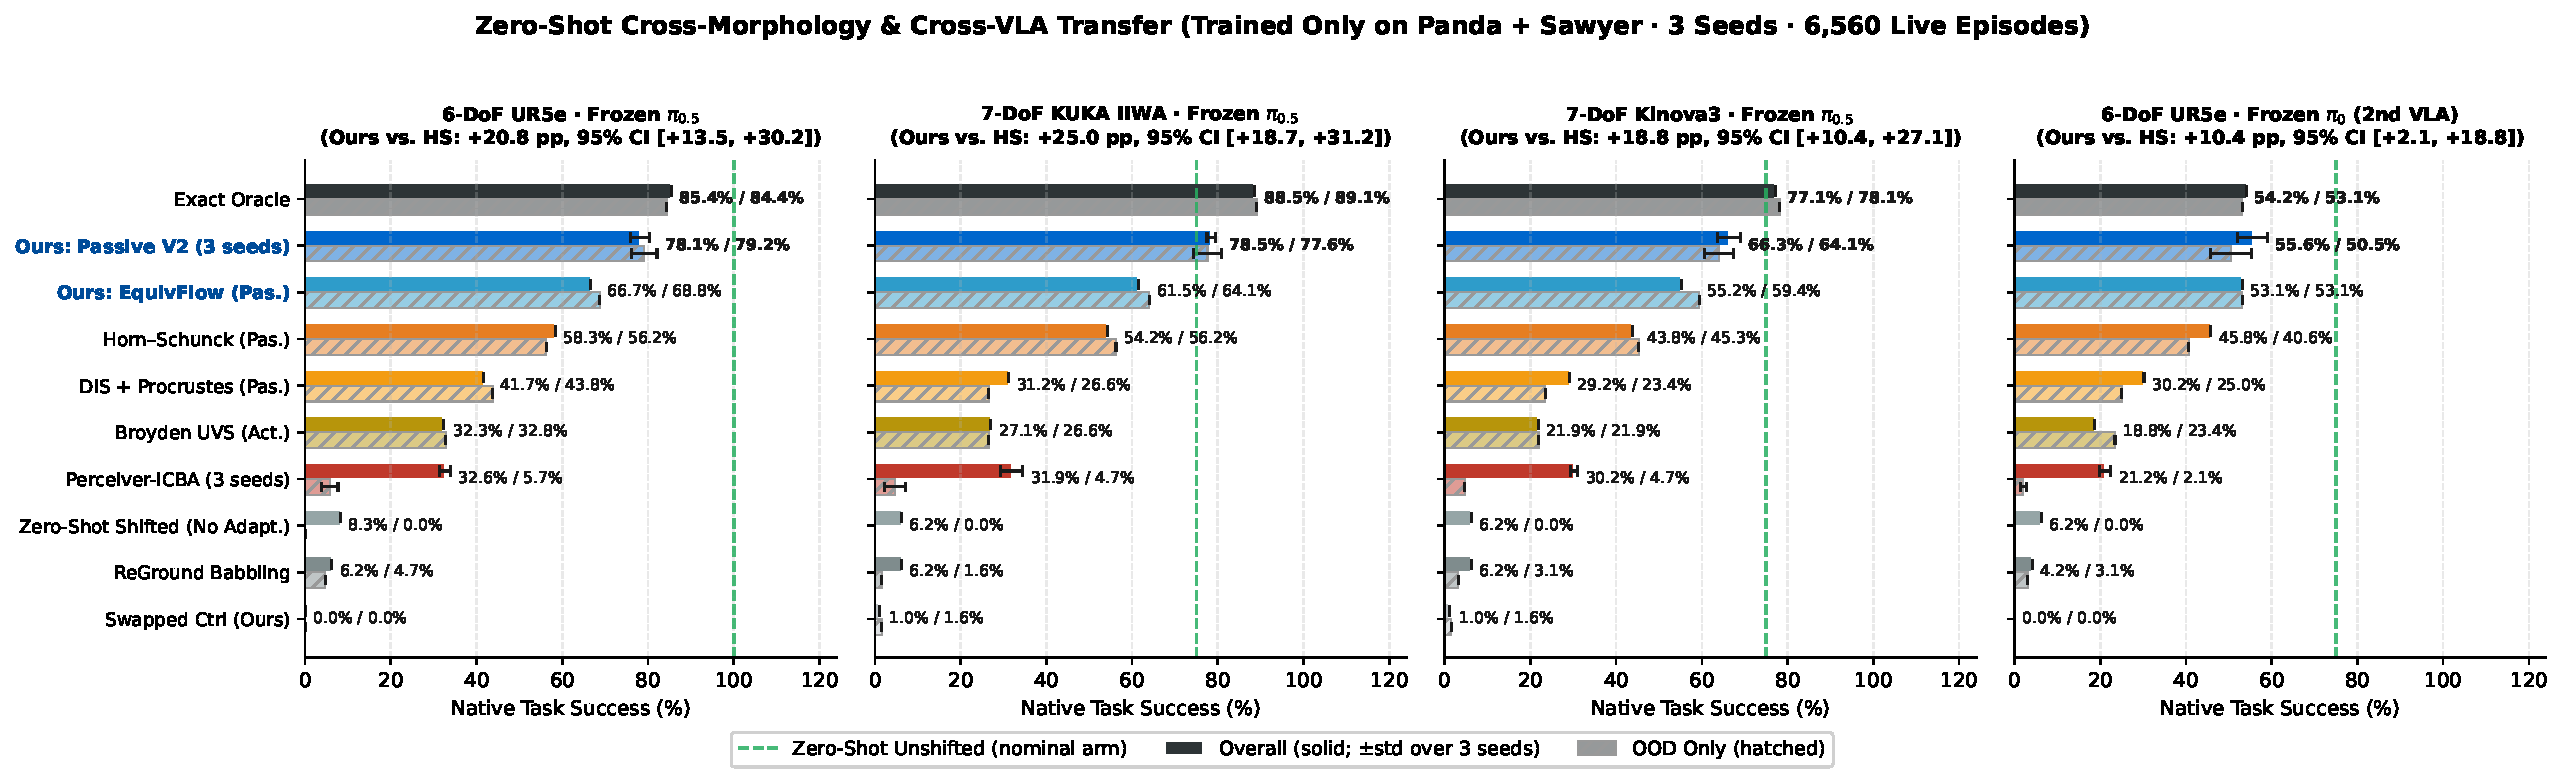
\includegraphics[width=\columnwidth]{figures/fig1_multiarm_multivla.pdf}
  \caption{\textbf{Single attempt and seed-matched retry.} The seed-41 reader either updates during the scored episode or starts it calibrated from 15 controls on an earlier layout. Each row uses the same 96 query resets and policy-noise draws for both protocols.}
  \label{fig:multiarm}
\end{figure}

A single-attempt controller must collect evidence while its uncorrected actions are already changing the scene. On a retry, the controller applies the prior estimate from the first action. We measure both protocols (Fig.~\ref{fig:multiarm}) and include an uncorrected retry under the same shifts (Table~\ref{tab:headline}). We then test which signals identify the rotation, how the learned reader transfers to unseen command settings, and how the estimate changes when the camera moves or joint kinematics supply the reference frame.

\section{Related Work}

\paragraph{Cross-embodiment VLAs and visual transfer.}
Generalist VLAs~\citep{brohan2023rt2,kim2024openvla,doshi2024scaling,black2025pi0,black2025pi05} transfer broadly across canonical robots but assume a consistent command interface. Mirage~\citep{chen2024mirage} and RoVi-Aug~\citep{chen2024roviaug} address visual appearance mismatch under known kinematics. We address an unknown command-frame rotation, gain, and gripper polarity, and we neither retrain the policy nor edit images.

\paragraph{In-context adaptation and online system identification.}
Online system identification~\citep{yu2017preparing,kumar2021rma,laskin2023algorithm} uses interaction histories to infer dynamics. In-context behavior adaptation (ICBA) trains a policy to use a Transformer encoding of commanded actions and observed motion~\citep{yang2026icba}. ReGround keeps a VLA frozen, learns dynamics from task-agnostic motor babbling and tracks intended motion under shifts including latency~\citep{siddique2026reground}. We evaluate two local proxies. One is a Perceiver~\citep{jaegle2022perceiverio} trained to predict interface factors. The other fits an affine map to command-frame proprioception. All reported outcomes for these comparators belong to the local implementations.

\paragraph{Geometric calibration.}
Hand--eye calibration~\citep{tsai1989handeye,park1994handeye} relates measured poses across frames. Uncalibrated visual servoing~\citep{jagersand1997uvs} estimates an image Jacobian, and dense inverse search (DIS) estimates optical flow~\citep{kroeger2016dis}. Procrustes alignment is classical~\citep{schonemann1966generalized,kabsch1976solution,umeyama1991least}. \citet{choy2020deep} already combined learned correspondence confidence with differentiable weighted Procrustes to register pairs of 3D scans. Here the quantities being aligned are issued commands and planar motion inferred from oblique video. Trace-level yaw supervision trains the motion readout and its weights through that alignment. The resulting equivariance concerns the command coordinates supplied to the solver, whereas equivariant policy networks impose symmetry on the policy itself~\citep{cohen2016group,wang2022equivariant}.

\section{Problem Formulation}

A frozen VLA outputs canonical relative end-effector commands $a_t = (\Delta p_t, \Delta r_t, u_t) \in [-1, 1]^7$. The target robot executes them with a hidden gripper sign, $u_t^{\text{phys}} = s\, u_t^{\text{cmd}}$, and a hidden motion transform:
\begin{align}
  \text{Planar:}\; & \Delta p_{t,xy}^{\text{phys}} = g\, R(\theta)\,\Delta p_{t,xy}^{\text{cmd}}, \label{eq:so2}\\
  \text{3D:}\; & \Delta p_t^{\text{phys}} = R\, D\,\Delta p_t^{\text{cmd}},\quad D = \operatorname{diag}(g_x, g_y, g_z), \label{eq:so3}
\end{align}
with $(\theta, g, s) \in [-\pi, \pi) \times \mathbb{R}_+ \times \{\pm 1\}$ in the planar case and $R \in SO(3)$ in the 3D case. The method observes a short history $\mathcal{H} = \{(I_k^{\text{before}}, I_k^{\text{after}}, \bar{a}_k, \Delta p_k^{\text{local}}, \Delta j_k)\}_{k=1}^K$ of camera frames, issued commands, end-effector displacements in the robot's command frame, and changes in gripper finger opening. Arm joint encoders are not an input. It estimates $(\hat{R}, \hat{D}, \hat{s})$ and wraps the frozen VLA with the inverse adapter $\bar{a}_t^{\text{issued}} = \hat{D}^{-1}\hat{R}^\top a_t^{\text{VLA}}$ (and $\hat{s}$ for the gripper). The planar wrapper also rotates the observed end-effector displacement from its reset position back into the policy frame.

\begin{proposition}[Command-frame displacements do not identify $R$]
\label{prop:unident}
Suppose end-effector displacements are measured in the robot's command frame, $\Delta p_k^{\text{local}} = R^\top \Delta p_k^{\text{world}}$, with $\Delta p_k^{\text{world}} = R D \bar{a}_k$ as in Eq.~\eqref{eq:so3}. Then $\Delta p_k^{\text{local}} = D\bar{a}_k$ for every $R \in SO(d)$. If the commands $\bar{a}_{1:K}$ are chosen independently of $R$ (for example a fixed probe sequence), the joint distribution of $(\bar{a}_k, \Delta p_k^{\text{local}})_{k \le K}$ does not depend on $R$, and the posterior over $R$ given these observations equals the prior. For a uniform prior on $\theta$ in the planar case, every estimator that uses only these observations has expected absolute angular error $90^\circ$.
\end{proposition}
\begin{proof}
Substitute $\Delta p_k^{\text{world}}$ into the definition: $R^\top R D \bar{a}_k = D\bar{a}_k$. With commands independent of $R$, the likelihood of the observations is the same for every $R$. For a uniform $\theta$ on the circle, the wrapped absolute error of any fixed estimate is uniform on $[0^\circ, 180^\circ]$, with mean $90^\circ$.
\end{proof}

\begin{remark}
The cancellation applies to displacements reported in the rotating frame and to commands chosen independently of $R$. Joint encoders with a kinematic model and known base frame, world-frame measurements, or calibrated camera geometry can supply an external reference. A policy acting on images can also choose commands that depend on $R$. The local displacements retain information about $D$ even when $R$ cancels.
\end{remark}

\begin{proposition}[Equivariance of the Procrustes step]
\label{prop:equiv}
Let $v_k \in \mathbb{R}^d$ and $w_k > 0$ be visual motion estimates and weights computed without access to the commands $\bar{a}_k$, and hold them fixed. Define $H = \sum_k w_k\, v_k (\hat{D}\bar{a}_k)^\top = U\Sigma V^\top$ and $\hat{R} = U \operatorname{diag}(1, \dots, 1, \det(UV^\top)) V^\top$.
\begin{enumerate}
  \item \textbf{Planar case.} With $D = gI_2$, $\hat\theta(\bar a, v) = \operatorname{atan2}\big(\sum_k w_k (\bar{a}_k \times v_k), \sum_k w_k (\bar{a}_k \cdot v_k)\big)$ satisfies $\hat\theta(R(\Delta\theta)^\top \bar a, v) = \hat\theta(\bar a, v) + \Delta\theta \pmod{2\pi}$ for every $\Delta\theta$, whenever the two sums are not both zero. This identity holds for every choice of training rotations. Training can still affect the motions and weights supplied to the solver.
  \item \textbf{3D case with known gains.} If $v_k = R D \bar{a}_k$ exactly, $\hat{D} = D$, and the commands $\{D\bar a_k\}$ span $\mathbb{R}^3$, then $\hat{R} = R$. Without gain pre-scaling, $H = R D \big(\sum_k w_k \bar{a}_k \bar{a}_k^\top\big)$, whose orthogonal factor generally differs from $R$ when $D$ is anisotropic.
\end{enumerate}
\end{proposition}
\begin{proof}
(1) Rotating $\bar a_k$ by $R(\Delta\theta)^\top$ rotates every 2D cross and dot product pair by $\Delta\theta$, which shifts the atan2 by $\Delta\theta$ modulo $2\pi$. (2) With pre-scaling, $H = R\,\big(\sum_k w_k\, D\bar a_k (D\bar a_k)^\top\big)$. This is $R$ times a symmetric positive-definite matrix, whose polar factor is $R$.
\end{proof}

\begin{remark}
The equivariance is with respect to rotations of the \emph{command} frame for a fixed camera. It is not invariance to the camera. The reader expresses $v_k$ in a frame fixed by the training camera pose, so rotating the camera rotates $v_k$ and the estimate $\hat\theta$ with it. We measure this in \S\ref{sec:limits}. Part 2 is a noiseless statement with known gains; it gives no guarantee with estimated gains or monocular motion estimates.
\end{remark}

On our 3D probe fixture, raw Procrustes without pre-scaling has $11.73^\circ$ rotational bias, and pre-scaling with the true gains removes it to numerical precision. With estimated gains, the residual bias grows with the gain error; we report the live 3D results in \S\ref{sec:so3}.

\begin{proposition}[Linear pooling in \texttt{EquivFlow}]
\label{prop:cardinal}
Let $v_k = H_\phi(I_0) \sum_{x,y} M_\psi(x, y)\, f_k(x, y)$, where $f_k$ is dense optical flow, $H_\phi(I_0)$ is a $2\times 2$ matrix that depends only on the first frame, and the mask $M_\psi$ depends only on rotation-invariant per-pixel features (flow magnitude, luminance change and gradient magnitudes, luminance, pixel coordinates). For a fixed mask, $v_k$ is linear in $f_k$. A rotation of the flow field that leaves the mask unchanged therefore rotates $\sum M_\psi f_k$ by the same angle, and the reader cannot learn a direction-specific mapping, such as snapping to the training directions.
\end{proposition}

Because the mask depends on $\|f_k\|$, linearity holds only conditionally on the mask, and the image-plane map approximates 3D motion only locally. Proposition~\ref{prop:cardinal} rules out direction-specific nonlinearities in the reader, but it does not guarantee accurate motion estimates.

\section{Method}
\label{sec:method}

We specify the three interface factors and their inverse. We train the reader from random initialization on 1,344 labeled Panda and Sawyer traces from 24 training tasks for the main planar experiment. At deployment its weights are frozen. It receives camera frames, issued commands and local robot measurements. It has no task or robot identifier. The visual estimate assumes the training camera pose relative to the robot base.
\begin{enumerate}
  \item \textbf{SymMeta.} Three stride-2 convolutions (48, 96, 96 channels) and a residual block encode a $64\!\times\!64$ map of DIS flow and magnitude, signed intensity change, RMS color change, two intensity gradients and pixel coordinates. Two learned spatial attention maps pool the $8\!\times\!8$ feature grid. A feedforward head reads the pooled features. It predicts planar motion $v_k^{\text{raw}}$, a confidence $w_k$, and a parallax coupling vector $u_{z,k}$. Subtracting the vertical-motion term,
  \[
    v_k = v_k^{\text{raw}} - \Delta z_k^{\text{local}}\, u_{z,k},
  \]
  compensates for parallax in the oblique view before weighted Procrustes (Prop.~\ref{prop:equiv}). Vertical displacement $\Delta z^{\text{local}}$ is invariant to planar rotations about $z$, so this correction preserves equivariance in the planar case. Two small MLPs estimate gain from issued translations and local displacements and gripper polarity from the gripper command, jaw motion and final opening (Appendix~\ref{sec:training-details}). The 3D variant outputs $v_k \in \mathbb{R}^3$ and per-axis log-gains, then applies gain-pre-scaled SVD Procrustes.
  \item \textbf{\texttt{EquivFlow}.} This variant implements Prop.~\ref{prop:cardinal}. A 7-channel pixel-attention CNN that sees no flow directions pools DIS flow through a learned $2\times 2$ matrix $H_0$, or a first-frame-conditioned $H_\phi(I_0) = H_0 + \Delta H_\phi(I_0)$. With an MLP reader trained on axis-aligned probe bursts, continuous OOD yaw error is $38.0^\circ$, because the reader snaps to the training directions. \texttt{EquivFlow} reduces this to $9.6^\circ$ (active probe) and $10.3^\circ$ (passive), measured offline. In live control it trails SymMeta (Table~\ref{tab:additional_baselines}), so we treat it as the structurally safer variant under sparse axis-aligned probes, not as the headline method.
\end{enumerate}


\begin{figure}[t]
  \centering\footnotesize
  \setlength{\fboxsep}{4pt}
  \fbox{\begin{minipage}{0.88\columnwidth}\centering
    \textbf{First attempt} \quad 3 chunks $\times$ 5 controls\\
    RGB frame pairs, issued commands, local motion and jaw width\\[2pt]
    $\downarrow$\\[-1pt]
    Visual reader $\to$ motion directions and confidence\\
    Local motion and gripper readers $\to$ gain and polarity\\[2pt]
    $\downarrow$\\[-1pt]
    Weighted Procrustes aligns motion to commands $\to \hat R$\\[2pt]
    $\downarrow$\\[-1pt]
    \textbf{Second attempt} \quad Frozen VLA $\to$ inverse action correction
  \end{minipage}}
  \caption{SymMeta estimates one command interface from the first attempt and applies it throughout the query episode. Training details appear in Appendix~\ref{sec:training-details}.}
  \label{fig:pipeline}
\end{figure}

\section{Experiments}

\subsection{Setup}
\label{sec:setup}

\paragraph{Benchmark.} We use the eight task identities held out for controlled studies in LIBERO-Pro2.0~\citep{liu2023libero,liberopro2026}: Spatial 0 and 8, Object 1 and 8, Goal 3 and 6, and Long 5 and 8 (zero-based IDs). We use their \texttt{BASE} scenes and cross each with our twelve command settings, giving 96 queries per arm--VLA pair. The holdout applies to reader training. The VLAs may have encountered these tasks during pretraining. The 7 training transforms are the nominal transform, yaw $\in \{90^\circ, 180^\circ, -90^\circ\}$, gain $\in \{0.65, 1.55\}$, and gripper inversion, each varying one factor. The 12 test transforms fall into three groups of four:
\begin{itemize}
  \item \emph{familiar}: nominal, yaw $90^\circ$, yaw $180^\circ$, gripper inversion;
  \item \emph{compositional OOD}: training factor values never combined in training, e.g.\ yaw $180^\circ$ with gain $0.65$ and inverted gripper;
  \item \emph{continuous OOD}: unseen yaws $\pm 45^\circ$ and $\pm 135^\circ$, combined with gains $0.75$, $1.0$, or $1.35$ and either gripper sign.
\end{itemize}
``OOD'' pools the 64 compositional and continuous queries. All arms are simulated in MuJoCo. A step is one control at 20\,Hz of simulated time.

\paragraph{Protocol.} For each task and command setting, the unadapted frozen VLA executes 15 controls on initial layout 11 (Attempt~1). All passive readers and training seeds share three five-control chunks from that trace. A fresh episode on layout 13 scores native success (Attempt~2). The calibrated retry starts with the estimated correction and holds it fixed. The uncorrected retry uses the identity wrapper on the same scheduled query. Active methods collect a separate 15-control probe. Support lasts 0.75\,s of simulated motion, excluding reset and inference time.

The single-attempt test starts uncorrected on layout 13 and updates from its own motion. Its first correction can take effect after ten controls. The seed-matched calibrated retry uses the same seed-41 checkpoint, query reset and policy-noise bank. Each protocol contributes one scored episode per query.

\paragraph{Statistics.} Learned methods (SymMeta, Perceiver) are trained with 3 seeds (41--43) and evaluated on all 96 queries per seed. The three seeds share the same 96 queries and support traces, so the reported mean $\pm$ standard deviation reflects reader-training variance only, and the independent units are the 8 tasks. Deterministic baselines are run once. We bootstrap paired differences by resampling eight whole tasks. For three-seed contrasts we first average the paired differences for each query. Appendix~\ref{sec:paired} reports per-seed gains and paired sign-flip tests at the query and task levels.

\paragraph{Baseline implementations.} The brightness-translation reader fits one global translation per frame pair by weighted least squares on brightness constancy, weighting pixels by absolute temporal intensity change. It computes no dense flow field. Both this reader and the DIS comparator project image motion to planar motion using nominal Panda and Sawyer active probes. Broyden updates its Jacobian on the target probe. The passive brightness-translation and learned readers share target traces, but differ in source supervision and in their gain and gripper estimators. Their native success difference compares the complete adapters. Our Perceiver proxy predicts the transform from the same support as SymMeta. Our affine proxy fits a ridge-regularized map from issued planar commands to local displacements and projects it onto a scaled rotation. It uses only the passive trace.

\paragraph{$\pi_0$ state encoding.} $\pi_0$ adds the end-effector axis-angle from \texttt{observation/state[3:6]} to its predicted actions. UR5e and Panda share the same downward gripper pose at reset. However, UR5e's MuJoCo quaternion lies on the opposite sign of the $SO(3)$ double cover (axis-angle $x = -3.133$ vs.\ $+3.141$), which produced a $2\pi$ jump that saturated the wrist command. Even the exact oracle succeeded on 0 of 96 queries. We canonicalize $q \equiv -q$ on the downward-gripper hemisphere in the $\pi_0$ state observation for every method, including the oracle. With this fix, the oracle reaches 54.2\%.

\subsection{Calibrating a Second Attempt}

\begin{table*}[t]
  \centering
  \caption{\textbf{Native success on eight held-out task identities under imposed command shifts.} The first four numeric columns count successes on 96 queries. The single attempt and calibrated retry use the same seed-41 SymMeta checkpoint. The uncorrected retry and the exact inverse use the same query schedule. The last two columns give calibrated retry success (\%, mean $\pm$ SD over reader seeds 41--43) on all settings and on the eight OOD shifts.}
  \label{tab:headline}
  \small
  \setlength{\tabcolsep}{4pt}
  \begin{tabular}{lrrrrrr}
    \toprule
    & & \multicolumn{2}{c}{SymMeta (seed 41)} & & \multicolumn{2}{c}{SymMeta retry (3 seeds)} \\
    \cmidrule(lr){3-4}\cmidrule(l){6-7}
    Arm (policy) & Uncorrected retry & Single attempt & Calibrated retry & Exact inverse & All 96 & OOD 64 \\
    \midrule
    UR5e ($\pi_{0.5}$)    & 8 & 20 & 76 & 82 & $78.1\pm2.3$ & $79.2\pm2.9$ \\
    IIWA ($\pi_{0.5}$)    & 6 & 26 & 76 & 85 & $78.5\pm1.0$ & $77.6\pm3.2$ \\
    Kinova3 ($\pi_{0.5}$) & 6 & 21 & 60 & 74 & $66.3\pm2.7$ & $64.1\pm3.4$ \\
    UR5e ($\pi_0$)        & 6 &  9 & 54 & 52 & $55.6\pm3.4$ & $50.5\pm4.8$ \\
    \bottomrule
  \end{tabular}
\end{table*}

\begin{figure*}[t]
  \centering
  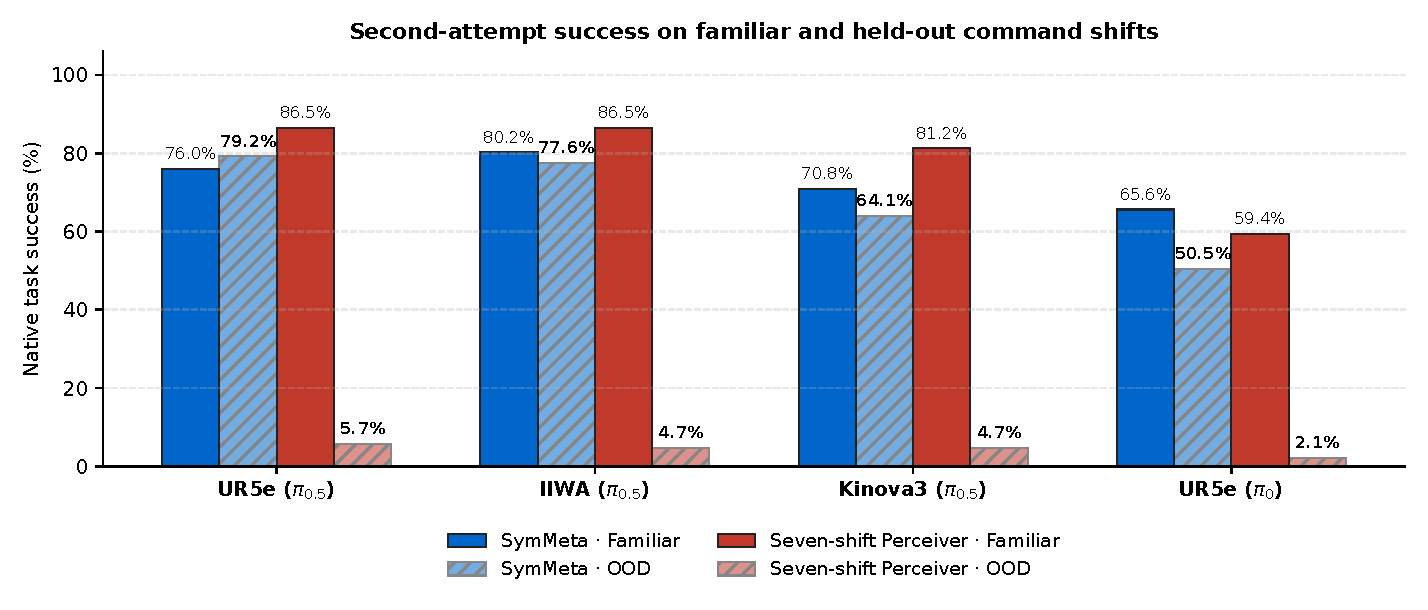
\includegraphics[width=0.98\textwidth]{figures/fig4_memorization_cliff_matrix.pdf}
  \caption{\textbf{Familiar vs.\ OOD success (3-seed means).} The local Perceiver reaches 59.4--86.5\% on familiar settings and 2.1--5.7\% on OOD settings. Each arm--policy pair has 32 familiar and 64 OOD queries.}
  \label{fig:cliff}
\end{figure*}

With one uninterrupted attempt, the seed-41 reader succeeds on 9--26 of 96 queries per panel. The seed-matched calibrated retry succeeds on 54--76, while an uncorrected retry succeeds on 6--8 (Table~\ref{tab:headline}). A retry changes both when correction begins and which trajectory supplies evidence. Replacing the support trace with one from a different command setting reduces calibrated retry success to 0--1\% (Appendix Table~\ref{tab:additional_baselines}).

\paragraph{What the visual reader contributes.} Across three seeds the calibrated retry gains 19.8, 24.3 and 22.6 percentage points over brightness-translation on the three $\pi_{0.5}$ arms. All eight task means favor SymMeta on each arm. On UR5e with $\pi_0$ the gain is 9.7 points and six tasks favor SymMeta (task-level $p=0.078$; Appendix~\ref{sec:paired}).

For a stronger control, we fit a six-coefficient projection of pooled DIS flow and vertical displacement on the same 1,344 Panda/Sawyer traces and yaw labels as the seed-41 reader. Both methods align three unit directions with equal weights and share gain and gripper estimates. On 64 OOD UR5e $\pi_{0.5}$ queries, learned and linear yaw errors were $6.53^\circ$ and $9.16^\circ$ (paired reduction $2.63^\circ$, 95\% task-bootstrap interval $[1.64,3.65]$). Fresh calibrated retries succeeded on 46 vs.\ 39 (+10.9 points, 95\% interval $[1.6,21.9]$). Six of seven net gains came from compositional shifts. This isolates the complete visual readout. Flow extraction, features and pooling differ. Appendix~\ref{sec:matchedflow} reports all outcomes.

\paragraph{Forward kinematics.} The FK reader uses additional information from encoder measurements for all six arm joints, their reset configuration and a trusted model of the UR5e and its gripper in a known base frame. It aligns the resulting world-frame tool displacements to the issued commands. On UR5e with $\pi_{0.5}$, we reran FK and the seed-41 visual reader on the same 96 query resets and policy-noise draws. Both used identical learned gain and gripper estimates. Changing only yaw gave 78/96 native successes for FK and 76/96 for vision (7 FK-only, 5 vision-only, 84 ties). FK minus vision was $+2.1$ percentage points (95\% task-cluster bootstrap interval $[-2.1,+7.3]$). FK reduced mean absolute yaw error from $6.67^\circ$ to $1.93^\circ$ overall and from $6.83^\circ$ to $2.02^\circ$ on the 64 OOD supports. The native-success interval admits effects in either direction.

\paragraph{Comparison to action adapters fitted on target demonstrations.}
We fit a linear or MLP action adapter to $K\in\{1,3,10\}$ successful demonstrations per shift on UR5e ($\pi_{0.5}$). Each demonstration uses the exact inverse transform. Across four OOD shifts the ten-demo sets contain 6,635 retained transitions, excluding failed collection attempts. Each fitted adapter serves all eight tasks on its shift. SymMeta instead uses 15 passive controls (0.75\,s) and a reset per query. On the same 32 task--transform pairs, the one-demo linear adapter succeeds on 28, SymMeta on 25, the oracle on 27 and brightness-translation on 18 (Fig.~\ref{fig:fewshot}). The separate runs match simulator reset seeds and layout 13. The seed-41 panel replays policy noise across methods; the adapter evaluator samples its own noise, so the three-success gap is descriptive. Both ten-demo adapters score 0/32 when transferred to the next shift (Table~\ref{tab:fewshot}).

\begin{table}[t]
  \centering
  \caption{UR5e ($\pi_{0.5}$) on four OOD shifts. Adapter and seed-41 rows share the 32 query resets. Policy noise differs across runs. $^\dagger$The adapter evaluator's own nominal control covers eight tasks.}
  \label{tab:fewshot}
  \scriptsize
  \setlength{\tabcolsep}{3pt}
  \resizebox{\columnwidth}{!}{%
  \begin{tabular}{lrrr}
    \toprule
    \textbf{Method on UR5e} & \textbf{Target demos} & \textbf{Same shift} & \textbf{Other shift} \\
    \midrule
    Unshifted VLA & 0 & 87.5\% (7/8)$^\dagger$ & --- \\
    Shifted, no adaptation & 0 & 0/32 & --- \\
    MLP adapter & $1/3/10$ & $18/25/28$ of 32 & 0/32 ($K{=}10$) \\
    Linear adapter & $1/3/10$ & $28/28/27$ of 32 & 0/32 ($K{=}10$) \\
    SymMeta (seed 41, same 32) & 0 & 78.1\% (25/32) & n/a \\
    brightness-translation (same 32) & 0 & 56.2\% (18/32) & n/a \\
    Oracle (same 32) & 0 & 84.4\% (27/32) & n/a \\
    \bottomrule
  \end{tabular}}
\end{table}

\subsection{Training-Shift Diversity and Capacity}
\label{sec:scaling}

Do learned encoders fail only for lack of training diversity or capacity? We collect 1,466 MuJoCo Attempt-1 trajectories on Panda and Sawyer covering up to 128 sampled interface transforms. We train five models at $M \in \{2, 4, 7, 16, 32, 64, 128\}$ training transforms with 3 seeds each (105 models). We evaluate each model offline on the 64 recorded UR5e OOD support traces. Table~\ref{tab:scaling} reports how well each model recovers the transform, not task success.

\begin{figure*}[t]
  \centering
  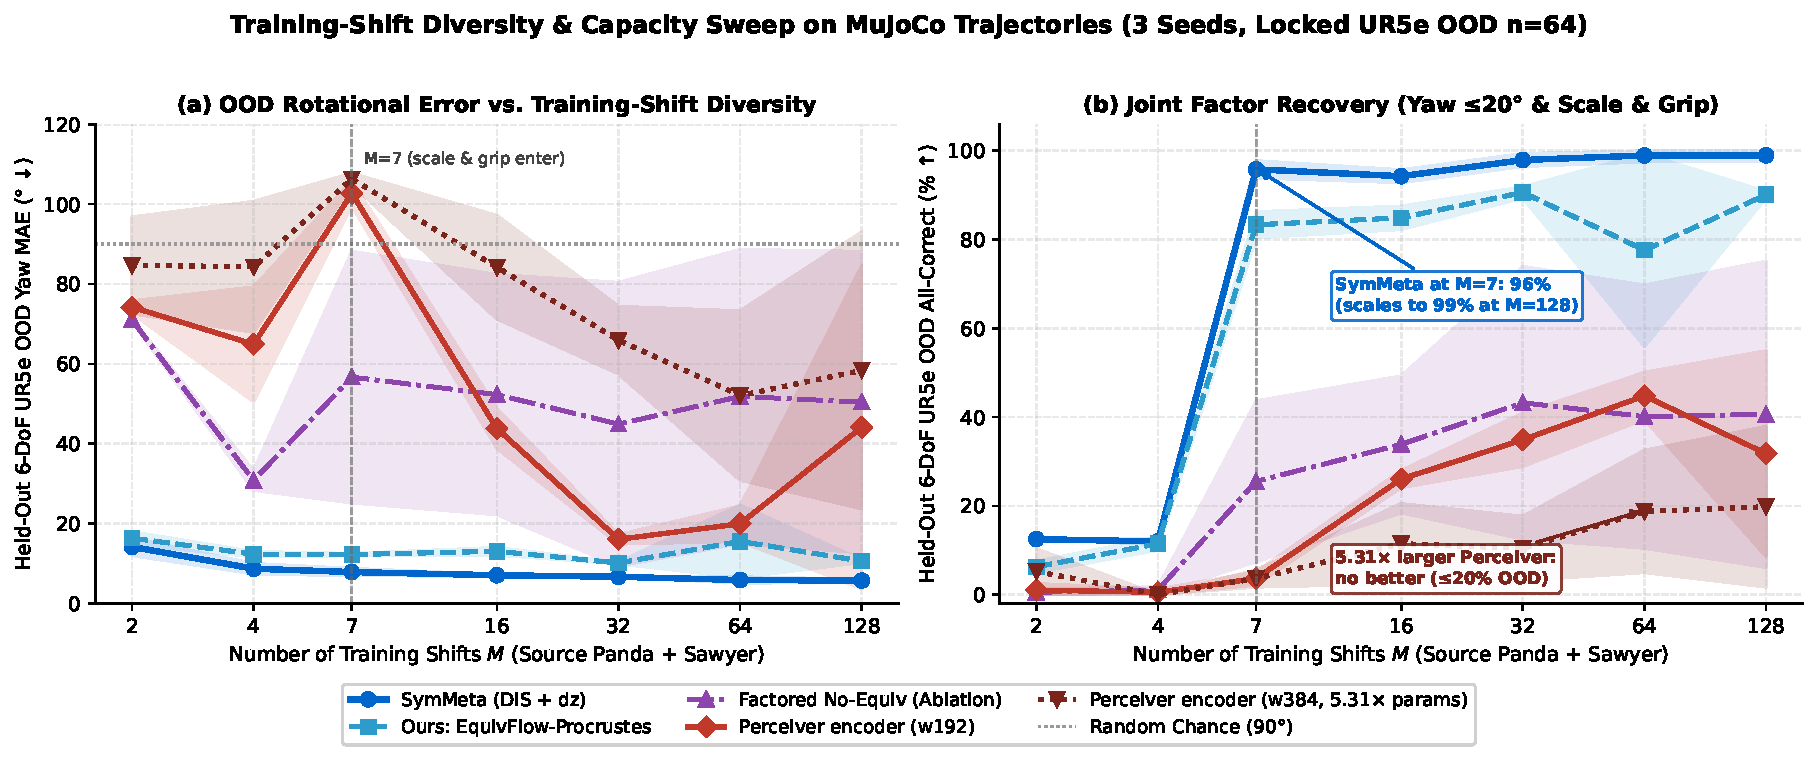
\includegraphics[width=0.98\textwidth]{figures/fig2_scaling_law.pdf}
  \caption{\textbf{Training-shift diversity and capacity sweep (5 models $\times$ 7 values of $M$ $\times$ 3 seeds; UR5e OOD queries).} Bands show one standard deviation across reader seeds. SymMeta reaches $7.9^\circ$ (96\% joint recovery) at $M{=}7$ and $5.7^\circ$ (99\%) at $M{=}128$. Non-equivariant models stay at or below 45\% across the sweep, with wide seed variance.}
  \label{fig:scaling}
\end{figure*}

Three patterns hold across the sweep. (1) Once gain and gripper variation enter at $M{=}7$, SymMeta recovers all factors on 96\% of OOD queries, and its yaw error keeps falling slowly up to $M{=}128$. (2) With 18$\times$ more training transforms ($M{=}128$ vs.\ $7$), the non-equivariant ablation and the w192 Perceiver still recover at most 45\% of OOD queries. The w192 Perceiver is not monotone in $M$, and its seed bands are wide. (3) The larger w384 Perceiver is never better than w192 from $M{=}16$ upward, and it has higher yaw error at every $M$. At $M{=}2$ its joint recovery is marginally higher (5\% vs.\ 1\%), and at $M{=}7$ the two tie.

\subsection{Support Length and 3D Rotations}

\paragraph{Support length (Fig.~\ref{fig:horizon_so3}A).}
On the UR5e OOD queries (3 seeds), SymMeta's yaw error is $12.7^\circ$ after 5 controls (0.25\,s), $7.4^\circ$ after 10, and $7.0^\circ$ after 15. With 15 controls, brightness-translation reaches $12.3^\circ$, DIS+Procrustes $24.1^\circ$, and the Perceiver baseline $95.6^\circ$. Removing the vertical-parallax correction raises SymMeta's error from $7.0^\circ$ to $12.1^\circ$.

\paragraph{Full 3D rotations with per-axis gains (Fig.~\ref{fig:horizon_so3}B).}
\label{sec:so3}
This extension is partial. The 3D reader is trained on 10 axis-aligned 3D transforms on Panda and Sawyer and tested on 12 held-out 3D transforms on UR5e ($n{=}96$). The test set includes oblique rotations, unequal gains $(0.65, 1.25, 1.40)$, and gripper inversion. It reaches 38.5\% success against an 88.5\% oracle: 68.8\% on familiar, 37.5\% on compositional, and 9.4\% on continuous $SO(3)$ transforms, with $24.5^\circ$ mean geodesic error. This beats the unadapted policy (7.3\%; $+31.2$ points, 95\% CI $[+19.8, +41.7]$, 31 wins / 1 loss) and the 3D command-frame affine baseline (4.2\%), but continuous 3D rotations remain largely unsolved (\S\ref{sec:limits}).

With a scripted motor in a second simulator, the parallax-corrected reader on xArm6 reaches 30.6\% success against a 66.7\% oracle (Appendix~\ref{sec:extra}).

\begin{figure*}[t]
  \centering
  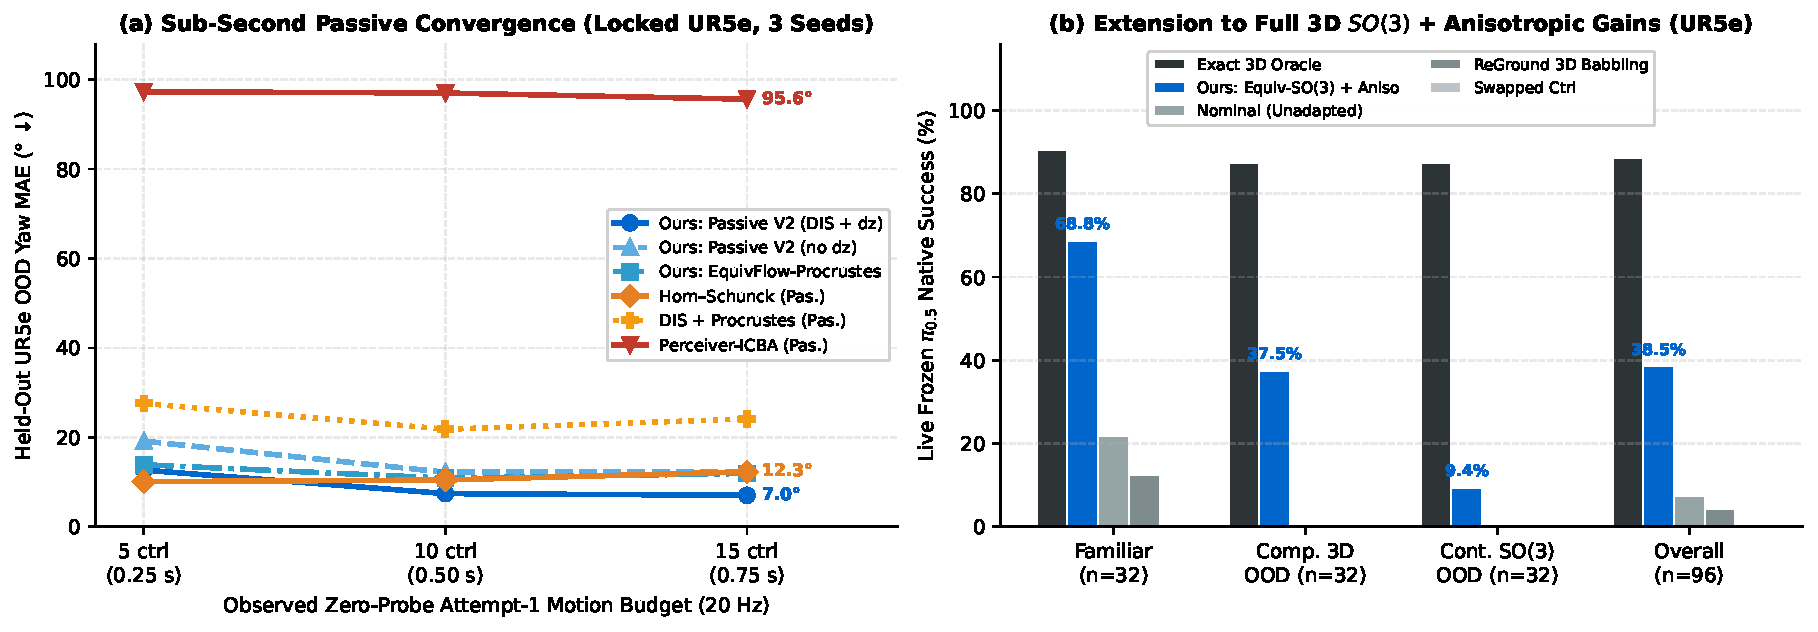
\includegraphics[width=0.98\textwidth]{figures/fig3_horizon_and_so3.pdf}
  \caption{\textbf{(A)} OOD yaw error vs.\ length of the passive support trace on UR5e (3 seeds). \textbf{(B)} Full 3D rotations with per-axis gains on UR5e ($n{=}96$): SymMeta improves on the unadapted policy and the 3D command-frame affine baseline but remains far below the oracle, especially on continuous $SO(3)$ transforms.}
  \label{fig:horizon_so3}
\end{figure*}

\subsection{LIBERO-Pro2.0 Visual and Camera Perturbations}

We test the \texttt{BASE}-trained SymMeta, without retraining, on 48 UR5e queries for each of five LIBERO-Pro2.0 visual and camera perturbations~\citep{liberopro2026}. We cross six command settings with each catalogue entry on all eight tasks~\citep[Table~15]{liberopro2026}. We use the object appearance (S13) variant that recolors objects, contrast or scene domain (S14) changes to palette and lighting, camera extrinsics (S15) offsets, camera image formation (S16) changes to field of view, and observation quality (S19) changes to RGB intensity and noise. Each of nine methods runs on all 240 queries (2,160 scored episodes). Table~\ref{tab:pro2} reports six methods. Figure~\ref{fig:pro2} compares the two passive readers with the exact inverse as a success reference.
Under \texttt{S15}, every method scores 0/48, including the exact inverse. Yaw error still distinguishes the estimates on these cases. On the four perturbations with a nonzero exact-inverse success rate, SymMeta reaches 69.3\% against a 76.0\% oracle and 56.8\% for brightness-translation.

\begin{table*}[t]
  \centering
  \caption{\textbf{Five LIBERO-Pro2.0 perturbations crossed with imposed command settings on UR5e ($\pi_{0.5}$, $n{=}48$ per row).} Cells give success (\%) and, for readers, mean yaw error in degrees. SymMeta is trained on \texttt{BASE} scenes only, while the Perceiver is retrained on Pro2 variants. All methods score 0/48 under \texttt{S15}. Over all 240 queries, the paired gain over brightness-translation is $+10.0$ points (95\% CI $[+4.2, +15.8]$, 35 wins / 11 losses).}
  \label{tab:pro2}
  \footnotesize
  \setlength{\tabcolsep}{4pt}
  \resizebox{\textwidth}{!}{%
  \begin{tabular}{lrrrrrr}
    \toprule
    \textbf{Variant} & \textbf{Oracle} & \shortstack[r]{\textbf{SymMeta}\\(passive)} & \shortstack[r]{\textbf{Brightness-}\\\textbf{translation} (passive)} & \shortstack[r]{\textbf{DIS + Proc.}\\(active)} & \shortstack[r]{\textbf{Local Perceiver}\\(active)} & \shortstack[r]{\textbf{Local affine}\\(passive)} \\
    \midrule
    \texttt{S13} object appearance & 85.4\% & \textbf{75.0\%} (5.87$^\circ$) & 62.5\% (8.58$^\circ$) & 45.8\% (14.29$^\circ$) & 27.1\% (71.78$^\circ$) & 8.3\% (96.03$^\circ$) \\
    \texttt{S14} contrast / scene domain & 85.4\% & \textbf{87.5\%} (5.85$^\circ$) & 68.8\% (9.82$^\circ$) & 54.2\% (16.02$^\circ$) & 29.2\% (72.69$^\circ$) & 8.3\% (88.70$^\circ$) \\
    \texttt{S16} camera image formation & 39.6\% & \textbf{35.4\%} (7.86$^\circ$) & 27.1\% (13.58$^\circ$) & 18.8\% (51.48$^\circ$) & 14.6\% (72.83$^\circ$) & 4.2\% (90.16$^\circ$) \\
    \texttt{S19} observation quality & 93.8\% & \textbf{79.2\%} (6.35$^\circ$) & 68.8\% (10.55$^\circ$) & 50.0\% (19.90$^\circ$) & 33.3\% (71.98$^\circ$) & 6.2\% (96.90$^\circ$) \\
    \midrule
    Excluding S15 ($n{=}192$) & 76.0\% & \textbf{69.3\%} & 56.8\% & --- & --- & --- \\
    \midrule
    \texttt{S15} camera extrinsics & 0.0\% & 0.0\% (\textbf{6.94$^\circ$}) & 0.0\% (8.43$^\circ$) & 0.0\% (22.03$^\circ$) & 0.0\% (72.27$^\circ$) & 0.0\% (88.21$^\circ$) \\
    All five ($n{=}240$) & 60.8\% & 55.4\% (6.57$^\circ$) & 45.4\% (10.19$^\circ$) & 33.8\% (24.75$^\circ$) & 20.8\% (72.31$^\circ$) & 5.4\% (92.00$^\circ$) \\
    \bottomrule
  \end{tabular}}
\end{table*}

\begin{figure*}[t]
  \centering
  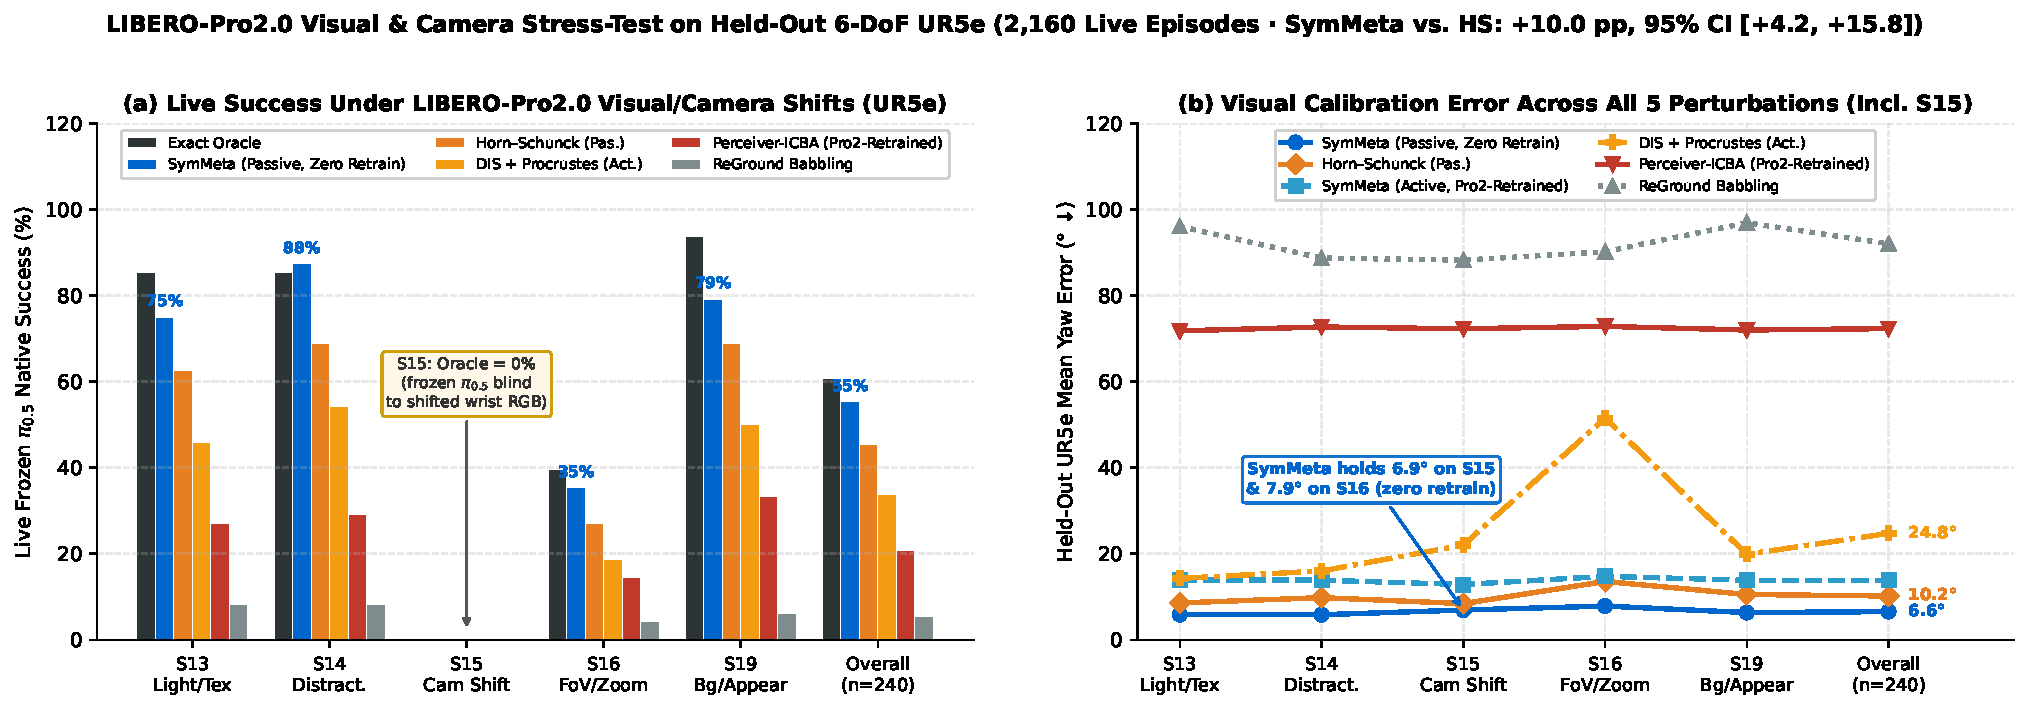
\includegraphics[width=0.98\textwidth]{figures/fig5_pro2_visual_stress.pdf}
  \caption{\textbf{Five LIBERO-Pro2.0 perturbations crossed with imposed command settings on UR5e.} \textbf{(A)} Success on each perturbation. \textbf{(B)} Mean yaw error, including \texttt{S15}, where the frozen VLA fails even with the exact transform.}
  \label{fig:pro2}
\end{figure*}

\section{Limitations}
\label{sec:limits}

\begin{enumerate}
  \item \textbf{Two attempts.} Calibration on an earlier layout gives the policy a corrected first action on the retry. Single-attempt results in Table~\ref{tab:headline} measure performance when the policy must estimate the interface while executing the task.
  \item \textbf{Camera pose.} The reader is not invariant to the camera. In an offline test on the 64 UR5e OOD support traces with the seed-41 reader, rotating the image by $\mp 90^\circ$ about the optical axis raised yaw error from $6.83^\circ$ to $84.5^\circ$ and $101.2^\circ$, and the estimate moved by about the roll angle on every trace. The brightness-translation reader behaved the same way ($12.3^\circ$ to $84.4^\circ$ and $101.6^\circ$). Orbiting the simulated camera by $\pm 30^\circ$ about the vertical on eight fresh trajectories shifted SymMeta's estimate by $28$--$30^\circ$. SymMeta therefore estimates the command rotation relative to the camera, and recovers the command-frame rotation only when the camera is mounted as in training. Task success under camera rotation is not measured.
  \item \textbf{Information available.} The visual reader assumes a fixed camera. FK needs measured joints, calibrated geometry and a known base frame. The native comparison holds gain and gripper estimates fixed and covers one arm--policy pair.
  \item \textbf{Simulation only.} All arms are simulated (MuJoCo and SAPIEN). We have not tested on physical hardware.
  \item \textbf{Shift model.} We model the interface as a global rotation, gain, and gripper sign on end-effector commands. Other differences between arms, such as workspace, dynamics, and joint limits, are left to the frozen VLA. The oracle results suggest it handles them for these arms.
  \item \textbf{Full 3D rotations.} With a single camera, out-of-plane rotations are poorly observed: $24.5^\circ$ geodesic error and 38.5\% success against an 88.5\% oracle. This motivates multi-view or wrist-camera depth.
  \item \textbf{Camera shifts that break the VLA.} Under \texttt{S15}, SymMeta has a mean yaw error of $6.94^\circ$. Both camera views change, and even the exact inverse gives 0/48 successes.
\end{enumerate}

\section{Conclusion}

On eight held-out LIBERO-Pro2.0 task identities in base scenes, a frozen policy can use a short trace to calibrate a second attempt under researcher-imposed planar command shifts. A fixed camera supplies the direction that command-frame displacements alone cannot identify. With the same reader seed and query schedule, success is substantially lower when calibration must take place within a single attempt. The evidence concerns the specified shift family, simulated arms and camera placement. Physical deployment and transfer across camera poses remain open.

\section*{Impact Statement}

This paper presents work whose goal is to advance the field of machine learning for robot control. Methods that let a pretrained policy run on a robot with an unknown command interface could lower the cost of deploying robots. They could also make it easier to run a policy on hardware it was never validated on. All results here are in simulation, and physical deployment would need its own safety testing.

\bibliography{references}
\bibliographystyle{icml2026}


\clearpage
\onecolumn
\appendix
\section{Additional transfer comparisons}
\begin{table}[!ht]
  \centering
  \caption{\textbf{Additional baselines and controls on the seed-41 panel ($n{=}96$ per row).} SymMeta here is the seed-41 checkpoint, so its numbers differ from the 3-seed means in Table~\ref{tab:headline}. The last column gives the paired difference to brightness-translation with a task-clustered 95\% bootstrap CI. Probe mode: Pas.\ = passive Attempt-1 trace, Act.\ = 15-control active probe.}
  \label{tab:additional_baselines}
  \footnotesize
  \setlength{\tabcolsep}{4pt}
  \resizebox{\textwidth}{!}{%
  \begin{tabular}{lrrrrrrr}
    \toprule
    \textbf{Arm (VLA), seed 41} & \textbf{SymMeta (Pas.)} & \textbf{EquivFlow (Pas.)} & \textbf{DIS+Proc.\ (Pas.)} & \textbf{Broyden UVS (Act.)} & \textbf{Affine (proprio.)} & \textbf{Swapped support} & \textbf{Gain [95\% CI]} \\
    \midrule
    UR5e ($\pi_{0.5}$) & 79.2\% & 66.7\% & 41.7\% & 32.3\% & 6.2\% & 0.0\% & $+20.8$ $[+13.5, +30.2]$ \\
    IIWA ($\pi_{0.5}$) & 79.2\% & 61.5\% & 31.2\% & 27.1\% & 6.2\% & 1.0\% & $+25.0$ $[+18.7, +31.2]$ \\
    Kinova3 ($\pi_{0.5}$) & 62.5\% & 55.2\% & 29.2\% & 21.9\% & 6.2\% & 1.0\% & $+18.8$ $[+10.4, +27.1]$ \\
    UR5e ($\pi_0$) & 56.2\% & 53.1\% & 30.2\% & 18.8\% & 4.2\% & 0.0\% & $+10.4$ $[+2.1, +18.8]$ \\
    \bottomrule
  \end{tabular}}
\end{table}

\begin{table}[!ht]
  \centering
  \caption{Controls for the calibrated retry. The nominal VLA runs once on each of eight tasks. The remaining columns use the imposed settings. The local Perceiver is summarized over seeds 41--43. Gain is the seed-average SymMeta success rate minus brightness-translation, with the smallest seed gain in parentheses. The uncorrected retry had zero OOD successes on every panel.}
  \label{tab:comparators}
  \small
  \begin{tabular}{lrrrrr}
    \toprule
    & \shortstack[r]{Nominal VLA\\(successes / 8)} & \shortstack[r]{Brightness-translation\\(all 96, \%)} & \multicolumn{2}{c}{Local Perceiver (\%)} & \shortstack[r]{SymMeta gain\\(pp)} \\
    \cmidrule(lr){4-5}
    Arm (policy) & & & All 96 & OOD 64 & Mean (min) \\
    \midrule
    UR5e ($\pi_{0.5}$)    & 8 & 58.3 & $32.6\pm1.3$ & $5.7\pm1.9$ & $+19.8$ ($+16.7$) \\
    IIWA ($\pi_{0.5}$)    & 6 & 54.2 & $31.9\pm2.6$ & $4.7\pm2.6$ & $+24.3$ ($+22.9$) \\
    Kinova3 ($\pi_{0.5}$) & 6 & 43.8 & $30.2\pm0.9$ & $4.7\pm0.0$ & $+22.6$ ($+18.8$) \\
    UR5e ($\pi_0$)        & 6 & 45.8 & $21.2\pm1.3$ & $2.1\pm0.7$ & $+9.7$ ($+5.2$) \\
    \bottomrule
  \end{tabular}
\end{table}

\begin{figure}[!ht]
  \centering
  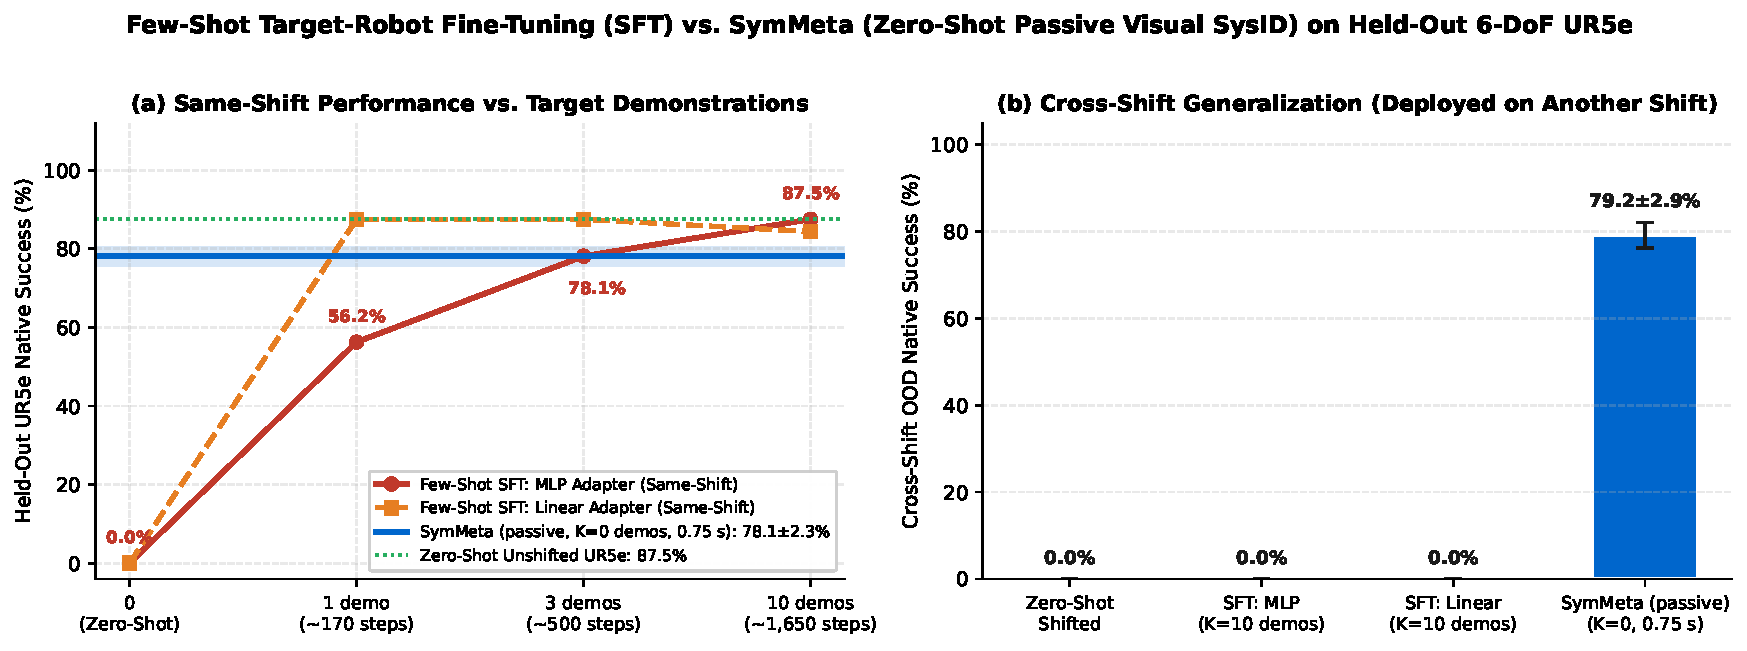
\includegraphics[width=0.95\textwidth]{figures/fig6_fewshot_sft_vs_sysid.pdf}
  \caption{\textbf{Demonstration-fitted action adapters vs.\ SymMeta on UR5e ($\pi_{0.5}$).} \textbf{(a)} Native successes by number of successful oracle demonstrations per shift. \textbf{(b)} Native successes on eight tasks at each of four OOD shifts. SymMeta, oracle and brightness-translation use the seed-41 panel. The one-demo linear adapter uses the same query resets with separate policy-noise draws.}
  \label{fig:fewshot}
\end{figure}

\clearpage
\section{Offline scaling and additional simulation results}
\label{sec:extra}
\begin{table}[!ht]
  \centering
  \caption{\textbf{Training-shift diversity and capacity sweep on UR5e OOD queries ($n{=}64$, 3 seeds per cell).} Each cell gives yaw MAE ($^\circ$, lower is better) and joint factor recovery (yaw within $20^\circ$, gain and gripper sign correct; higher is better). For $M \le 4$ only yaw varies, so joint recovery is near zero for every model by construction.}
  \label{tab:scaling}
  \footnotesize
  \setlength{\tabcolsep}{4pt}
  \resizebox{\textwidth}{!}{%
  \begin{tabular}{lrrrrrrr}
    \toprule
    \textbf{Model} & $M{=}2$ & $M{=}4$ & $M{=}7$ & $M{=}16$ & $M{=}32$ & $M{=}64$ & $M{=}128$ \\
    \midrule
    \textbf{SymMeta} & 14.2$^\circ$ (12\%) & \textbf{8.7$^\circ$} (12\%) & \textbf{7.9$^\circ$ (96\%)} & \textbf{7.1$^\circ$ (94\%)} & \textbf{6.7$^\circ$ (98\%)} & \textbf{5.9$^\circ$ (99\%)} & \textbf{5.7$^\circ$ (99\%)} \\
    \texttt{EquivFlow} & 16.4$^\circ$ (6\%) & 12.3$^\circ$ (11\%) & 12.2$^\circ$ (83\%) & 13.1$^\circ$ (85\%) & 10.1$^\circ$ (91\%) & 15.6$^\circ$ (78\%) & 10.6$^\circ$ (90\%) \\
    Factored, no equivariance (ablation) & 71.0$^\circ$ (1\%) & 30.8$^\circ$ (1\%) & 56.7$^\circ$ (26\%) & 52.3$^\circ$ (34\%) & 44.9$^\circ$ (43\%) & 51.8$^\circ$ (40\%) & 50.4$^\circ$ (41\%) \\
    Perceiver, w192 & 74.2$^\circ$ (1\%) & 64.9$^\circ$ (1\%) & 102.7$^\circ$ (4\%) & 43.8$^\circ$ (26\%) & 16.1$^\circ$ (35\%) & 20.0$^\circ$ (45\%) & 44.1$^\circ$ (32\%) \\
    Perceiver, w384 (5.31$\times$ params) & 84.7$^\circ$ (5\%) & 84.3$^\circ$ (0\%) & 106.3$^\circ$ (4\%) & 84.2$^\circ$ (11\%) & 65.9$^\circ$ (10\%) & 52.1$^\circ$ (19\%) & 58.4$^\circ$ (20\%) \\
    \bottomrule
  \end{tabular}}
\end{table}

\paragraph{Second simulator: ManiSkill3 / SAPIEN.}
In ManiSkill3/SAPIEN~\citep{tao2025maniskill3}, we train the reader on Panda and Fetch and evaluate the xArm6 with a scripted motor. The SymMeta reader with vertical-motion correction succeeds on 22/72 starts, including 11/48 held-out starts and 0/24 continuous-angle starts. The exact-transform oracle succeeds on 48/72. Removing the correction gives 5/72. These results limit the evidence for transfer across simulators. In a separate 3-seed LIBERO-Pro2.0 UR5e audit (576 episodes per method), a monolithic Transformer given continuous transform augmentation and twice the training steps reaches $13.8 \pm 9.2\%$ OOD success, and RMA-GRU reaches $11.5 \pm 0.7\%$.

\paragraph{Visual-perturbation panel.}
The nine methods comprise the exact oracle, unadapted policy, passive \texttt{BASE}-trained SymMeta, active camera-conditioned EquivFlow, active Pro2-trained SymMeta, passive brightness-translation, active DIS+Procrustes, command-frame affine fit and active Pro2-trained Perceiver.


\section{Paired native task success}
\label{sec:paired}
 We matched SymMeta and the source-calibrated brightness-translation reader on each held-out task identity, imposed interface, scheduled reset and simulator seed. We first computed the paired success difference separately for each checkpoint, then averaged those differences within query. Each panel contributes 96 queries over eight tasks. The 64 held-out queries use compositional or continuous-angle shifts.

\begin{table}[H]
\centering\small
\caption{Native success gains in percentage points. The three gains are ordered by reader seed (41, 42, 43). The interval and two-sided $p$-values refer to the seed-average contrast.}
\begin{tabular}{llrrrrr}
\hline
Arm (policy) & Queries & Gains by seed & Mean & 95\% task interval & $p_{\rm query}$ & $p_{\rm task}$ \\
\hline
UR5e ($\pi_{0.5}$) & All 96 & +20.8 / +16.7 / +21.9 & +19.8 & [+11.8, +31.2] & $7.15\times10^{-5}$ & 0.0078 \\
UR5e ($\pi_{0.5}$) & Held-out 64 & +25.0 / +18.8 / +25.0 & +22.9 & [+14.6, +33.3] & $0.00046$ & 0.0078 \\
IIWA ($\pi_{0.5}$) & All 96 & +25.0 / +25.0 / +22.9 & +24.3 & [+16.7, +31.9] & $3.75\times10^{-6}$ & 0.0078 \\
IIWA ($\pi_{0.5}$) & Held-out 64 & +25.0 / +21.9 / +17.2 & +21.4 & [+14.6, +28.6] & $0.000762$ & 0.0078 \\
Kinova3 ($\pi_{0.5}$) & All 96 & +18.8 / +25.0 / +24.0 & +22.6 & [+14.9, +29.9] & $1.67\times10^{-6}$ & 0.0078 \\
Kinova3 ($\pi_{0.5}$) & Held-out 64 & +14.1 / +20.3 / +21.9 & +18.8 & [+8.9, +28.6] & $0.00126$ & 0.0156 \\
UR5e ($\pi_0$) & All 96 & +10.4 / +5.2 / +13.5 & +9.7 & [+1.7, +19.4] & $0.0901$ & 0.0781 \\
UR5e ($\pi_0$) & Held-out 64 & +14.1 / +3.1 / +12.5 & +9.9 & [-3.1, +22.9] & $0.17$ & 0.2500 \\
\hline
\end{tabular}
\end{table}

For a single seed the exact query test flips the discordant binary pairs. For the seed average it flips the signed mean difference once per query, retaining its magnitude and the shared comparator. The task sensitivity enumerates all $2^8$ whole-task sign assignments. Each test assumes sign symmetry and independent flips at its stated unit. The percentile interval resamples eight whole tasks with replacement, conditional on the three checkpoints. All $p$-values are unadjusted. The eight fixed tasks limit generalization. On the full panel all eight task means favor SymMeta for each $\pi_{0.5}$ arm. On UR5e with $\pi_0$, six tasks favor SymMeta and two favor brightness-translation.


\subsection{Linear flow with matched source supervision}
\label{sec:matchedflow}
The linear reader maps two pooled DIS-flow components and measured vertical displacement to a planar vector. Both readers use the same 1,344 labeled source traces, 96 target supports and equal-weight yaw solver. For the 32 compositional shifts the learned reader reduced yaw error by $4.96^\circ$ (95\% task-bootstrap interval $[2.52,7.80]$). For the 32 continuous-angle shifts the reduction was $0.30^\circ$ ($[-2.40,2.90]$). Each query in Table~\ref{tab:matchedflow} uses the same reset, noise, prompt and opening policy proposal across readers. The learned arm here uses equal weights. The seed-41 headline uses the reader's original weights.

\begin{table}[h]
\centering\small
\caption{Native successes for the learned and linear readouts with matched source labels and target solver. The last two columns count pairs won by only one reader.}
\label{tab:matchedflow}
\setlength{\tabcolsep}{3pt}
\begin{tabular}{lrrrrr}
\toprule
Settings & Pairs & Learned & Linear & Lrn. only & Lin. only \\
\midrule
All & 96 & 70 & 62 & 14 & 6 \\
Held-out & 64 & 46 & 39 & 11 & 4 \\
Compositional & 32 & 23 & 17 & 8 & 2 \\
Continuous angle & 32 & 23 & 22 & 3 & 2 \\
Familiar & 32 & 24 & 23 & 3 & 2 \\
\bottomrule
\end{tabular}
\end{table}

\section{Reader training and model sizes}
\label{sec:training-details}
\paragraph{Planar reader.} The training set contains 1,344 passive traces: two source arms (Panda and Sawyer), 24 tasks, four initial states and seven interface transforms. Each trace supplies three five-control chunks. The simulator provides one yaw $\theta$, gain $g$ and gripper sign $s$ for the entire trace. We normalize the predicted yaw pair $(\hat c,\hat s_\theta)$ and train with the batch mean of
\[
  1-\hat c\cos\theta-\hat s_\theta\sin\theta
  +(\widehat{\log g}-\log g)^2
  +\operatorname{BCEWithLogits}(\hat h,\mathbf{1}[s>0]).
\]
All three losses have unit weight. For each checkpoint we sample 64 traces uniformly with replacement per update. We use AdamW for 3,500 updates with gradient-norm clipping at 1, weight decay $10^{-4}$ and cosine learning-rate decay from $10^{-3}$ to $5\times10^{-5}$. The headline Perceiver uses the same training data, loss and schedule.

\paragraph{Inputs and architecture.} The visual encoder processes $64\times64$ image pairs. Its nine channels are horizontal and vertical DIS flow, flow magnitude, signed mean-intensity change, RMS RGB change, the two gradients of temporally averaged intensity, and two pixel coordinates. Three $3\times3$ stride-two convolutions have 48, 96 and 96 channels, with a two-convolution residual block between stages two and three. Two spatial softmax pools produce 192 features, projected to 96 with SiLU activations in the encoder. A $96$--$192$--$96$--$5$ MLP predicts planar motion, a confidence logit and two parallax coefficients. The yaw loss reaches all five outputs through the alignment. Confidence is $\operatorname{softplus}(\ell_k)+10^{-4}$ on valid chunks. The vertical projection combines learned global and chunk-specific coefficients and multiplies local vertical motion in centimetres. Only the product of chunk weight and motion vector enters the yaw fit. Their individual magnitudes therefore lack a separate interpretation as calibrated reliability or speed. A $5$--$64$--$64$--$2$ gain head uses signed command and displacement, their magnitudes and a stabilized log-magnitude ratio. A $4$--$48$--$48$--$2$ gripper head uses gripper command, jaw change, final width and negative command times width change. Each head predicts a value and its pooling weight.

\paragraph{Perceiver capacity.} The headline model has 2,122,950 parameters, eight latents, 32 positional slots and attention width 192. The width-192 scaling model uses 24 slots and has 2,121,414 parameters. The width-384 model has 11,274,374 parameters, 16 latents, five self-attention blocks and eight heads. The larger configuration has 5.31 times as many parameters as the smaller scaling model.

\paragraph{Three-dimensional reader.} A separate seed-41 reader trains on 960 active probes from the two source arms, 24 tasks, two initial states and ten transforms. Six signed-axis bursts supply five controls each. A $96$--$128$--$64$--$4$ head outputs a three-vector and a confidence logit per chunk. This branch uses the visual vector directly and bypasses the planar vertical-motion correction. Estimated per-axis gains, clipped to $[0.25,4]$, rescale the commands before weighted SVD alignment. Its loss adds $\|\hat R-R\|_F^2/4$, mean squared log-gain error across axes and polarity cross-entropy. Training uses 3,000 AdamW updates, batch size 64 and cosine decay from 0.0015 to 0.000075 with the planar clipping and weight decay.

\end{document}
